% LTeX: language=en-US



\documentclass[draft,grl]{agutexSI2019}\usepackage[]{graphicx}\usepackage[]{xcolor}
% maxwidth is the original width if it is less than linewidth
% otherwise use linewidth (to make sure the graphics do not exceed the margin)
\makeatletter
\def\maxwidth{ %
  \ifdim\Gin@nat@width>\linewidth
    \linewidth
  \else
    \Gin@nat@width
  \fi
}
\makeatother

\definecolor{fgcolor}{rgb}{0.345, 0.345, 0.345}
\newcommand{\hlnum}[1]{\textcolor[rgb]{0.686,0.059,0.569}{#1}}%
\newcommand{\hlstr}[1]{\textcolor[rgb]{0.192,0.494,0.8}{#1}}%
\newcommand{\hlcom}[1]{\textcolor[rgb]{0.678,0.584,0.686}{\textit{#1}}}%
\newcommand{\hlopt}[1]{\textcolor[rgb]{0,0,0}{#1}}%
\newcommand{\hlstd}[1]{\textcolor[rgb]{0.345,0.345,0.345}{#1}}%
\newcommand{\hlkwa}[1]{\textcolor[rgb]{0.161,0.373,0.58}{\textbf{#1}}}%
\newcommand{\hlkwb}[1]{\textcolor[rgb]{0.69,0.353,0.396}{#1}}%
\newcommand{\hlkwc}[1]{\textcolor[rgb]{0.333,0.667,0.333}{#1}}%
\newcommand{\hlkwd}[1]{\textcolor[rgb]{0.737,0.353,0.396}{\textbf{#1}}}%
\let\hlipl\hlkwb

\usepackage{framed}
\makeatletter
\newenvironment{kframe}{%
 \def\at@end@of@kframe{}%
 \ifinner\ifhmode%
  \def\at@end@of@kframe{\end{minipage}}%
  \begin{minipage}{\columnwidth}%
 \fi\fi%
 \def\FrameCommand##1{\hskip\@totalleftmargin \hskip-\fboxsep
 \colorbox{shadecolor}{##1}\hskip-\fboxsep
     % There is no \\@totalrightmargin, so:
     \hskip-\linewidth \hskip-\@totalleftmargin \hskip\columnwidth}%
 \MakeFramed {\advance\hsize-\width
   \@totalleftmargin\z@ \linewidth\hsize
   \@setminipage}}%
 {\par\unskip\endMakeFramed%
 \at@end@of@kframe}
\makeatother

\definecolor{shadecolor}{rgb}{.97, .97, .97}
\definecolor{messagecolor}{rgb}{0, 0, 0}
\definecolor{warningcolor}{rgb}{1, 0, 1}
\definecolor{errorcolor}{rgb}{1, 0, 0}
\newenvironment{knitrout}{}{} % an empty environment to be redefined in TeX

\usepackage{alltt}

\usepackage{graphicx}
\setkeys{Gin}{draft=false} % Allow figure display.

\usepackage{color}
\newcommand*{\todo}[1]{\textbf{\textcolor{red}{(#1)}}}

\authorrunninghead{RAUPACH AND ALDRIDGE}
\titlerunninghead{CHANGES IN DAMAGING HAIL IN AUSTRALIA}

\authoraddr{Corresponding author: T. H. Raupach,
UNSW Sydney Climate Change Research Centre,
Mathews Building Level 4, 
UNSW Sydney, 
New South Wales 2052,
Australia
(timothy.h.raupach@gmail.com)}
\IfFileExists{upquote.sty}{\usepackage{upquote}}{}
\begin{document}

\title{Supporting Information for ``Changes in damaging hail in major Australian cities with global warming''}
% % %DOI: 10.1002/%insert paper number here%

\authors{Timothy H. Raupach\affil{1,2,3}, Joanna Aldridge\affil{4,5}}

\affiliation{1}{UNSW Institute for Climate Risk and Response, 
                UNSW Sydney, New South Wales, Australia}
\affiliation{2}{UNSW Climate Change Research Centre, 
                UNSW Sydney, New South Wales,  Australia}
\affiliation{3}{ARC Centre of Excellence for Climate Extremes, 
                Sydney, New South Wales,  Australia}
\affiliation{4}{School of Geosciences, University of Sydney, 
                Sydney, New South Wales,  Australia}
\affiliation{5}{QBE Australia, Sydney, 
                New South Wales, Australia}

\begin{article}

\noindent\textbf{Contents of this file}
\begin{enumerate}
    \item Figures S1 to S8.
    \item Tables S1 to S2.
\end{enumerate}

\clearpage

\bibliography{../main/library}

\end{article}

\clearpage

\begin{figure}[!h]
    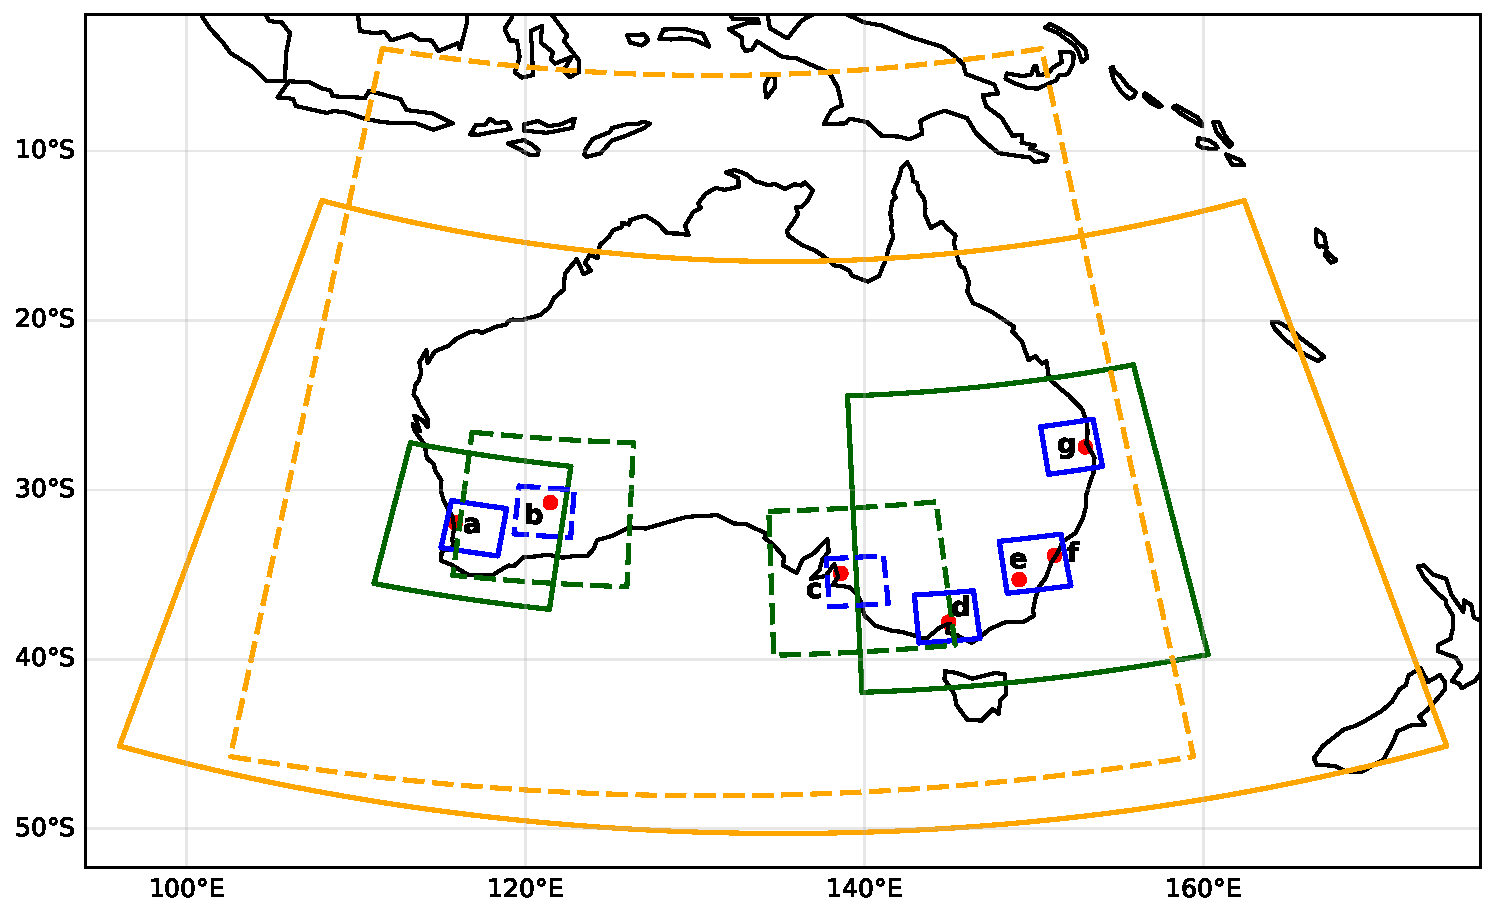
\includegraphics[width=\textwidth]{figures/domains}
    \caption{Approximate extents of the model domains on a map of Australia. The coarse-resolution domains are in yellow, medium-resolution domains in dark green, and fine-resolution domains in blue. The solid and dotted lines group the two sets of nested domains that were calculated together. Approximate city locations (with city extents not shown) are marked with red points for Perth (a), Kalgoorlie (b), Adelaide (c), Melbourne (d), Canberra (e), Sydney (f), and Brisbane (g).}
    \label{fig:domains}
\end{figure}

\begin{figure}[!ht]
    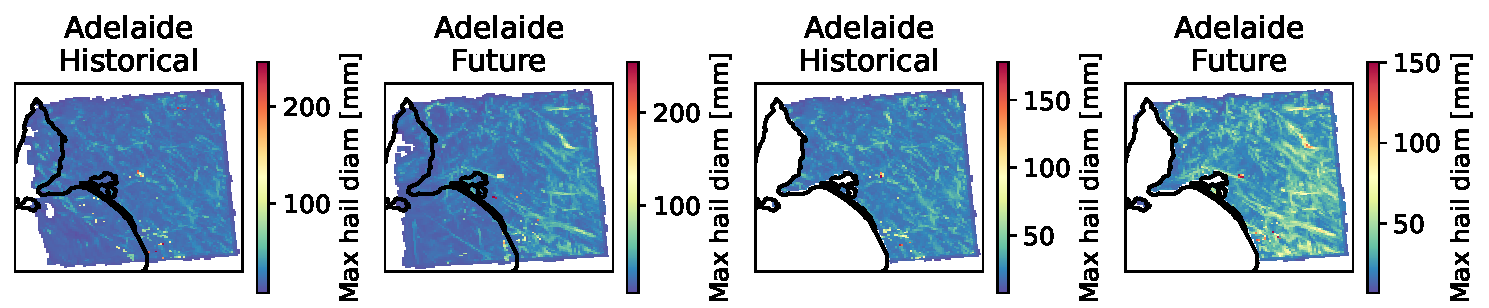
\includegraphics[width=\textwidth]{figures/maxes_Adelaide_hailcast_diam_max}
    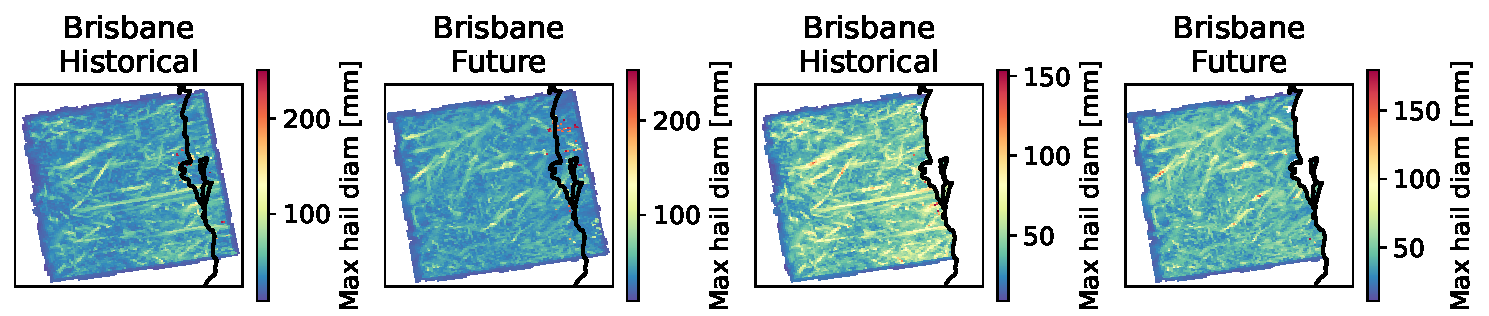
\includegraphics[width=\textwidth]{figures/maxes_Brisbane_hailcast_diam_max}
    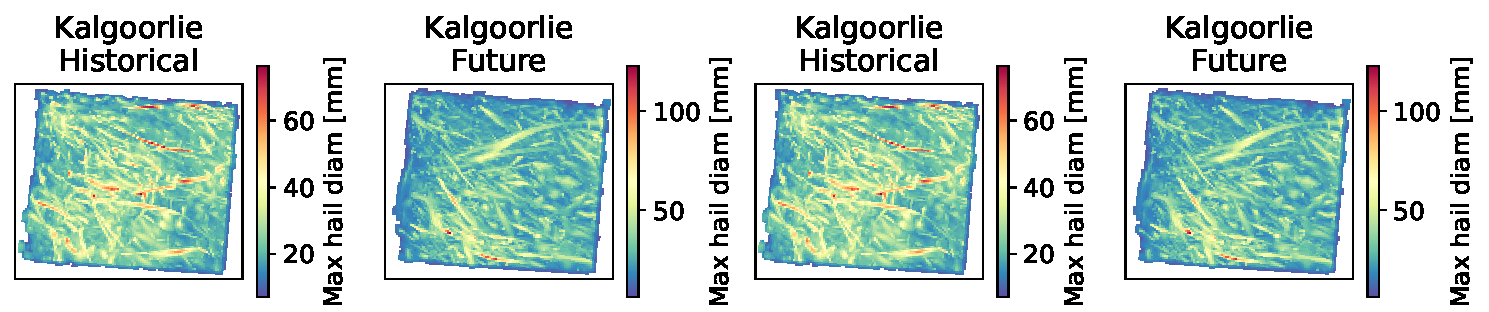
\includegraphics[width=\textwidth]{figures/maxes_Kalgoorlie_hailcast_diam_max}
    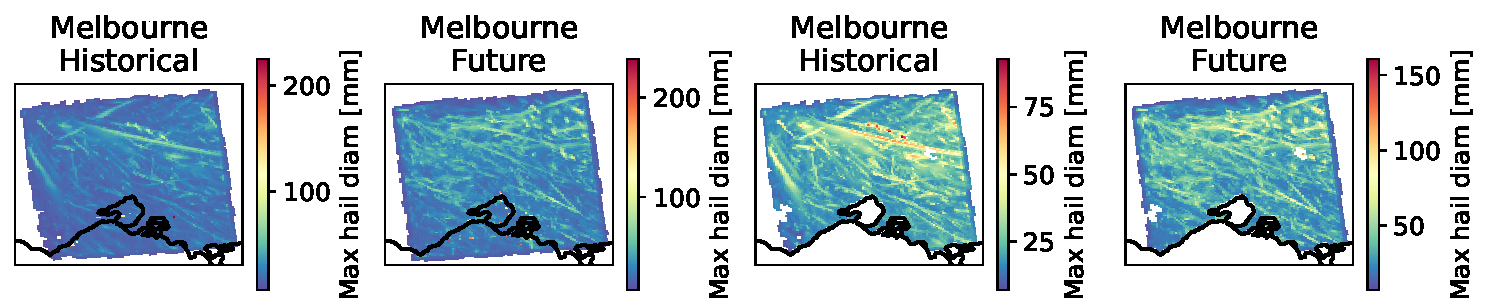
\includegraphics[width=\textwidth]{figures/maxes_Melbourne_hailcast_diam_max}
    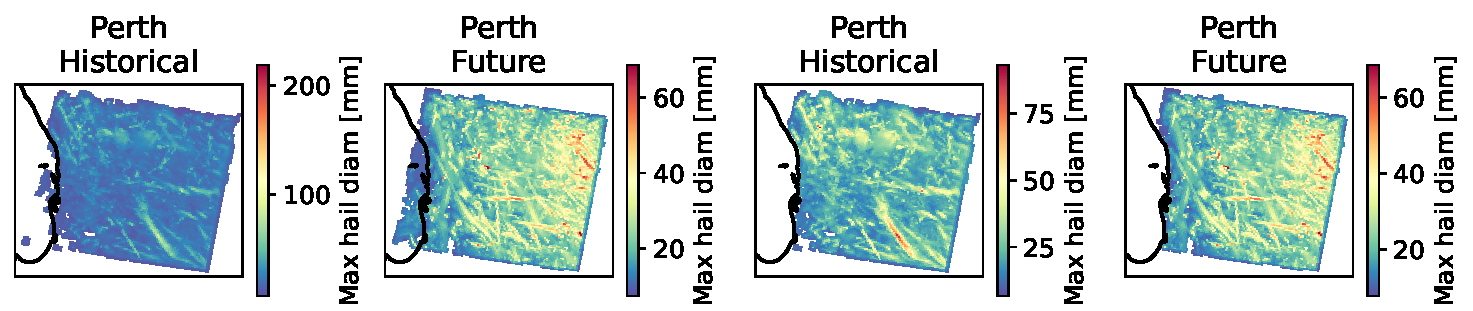
\includegraphics[width=\textwidth]{figures/maxes_Perth_hailcast_diam_max}
    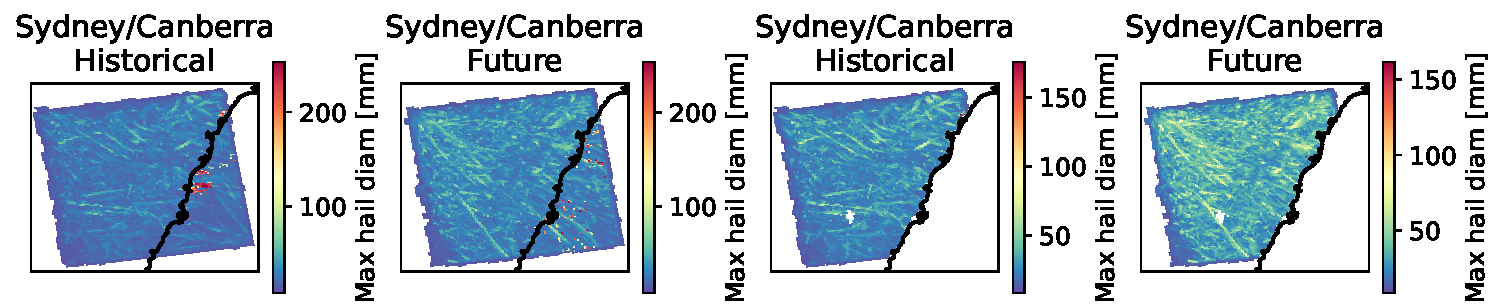
\includegraphics[width=\textwidth]{figures/maxes_Sydney_Canberra_hailcast_diam_max}
    \caption{Maximum hail size diameters for the Adelaide, Brisbane, Kalgoorlie, Melbourne, Perth, and Sydney/Canberra domains under the historical and future scenarios, with and without ocean areas removed.}
    \label{fig:maxes_with_removed_pts}
\end{figure}

\begin{figure}[!ht]
    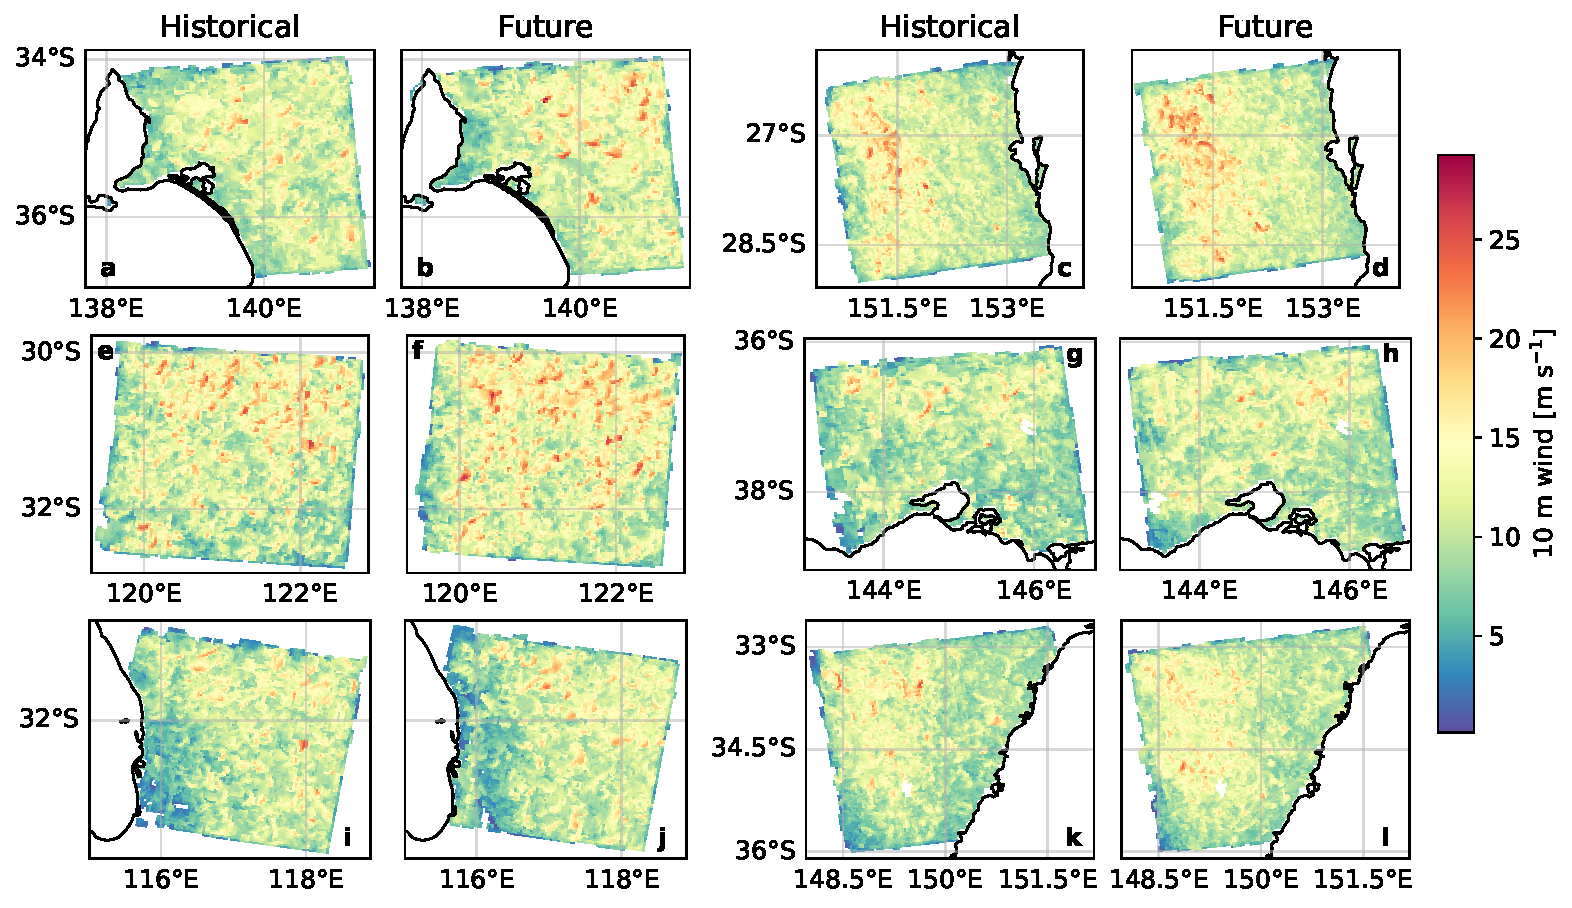
\includegraphics[width=\textwidth]{figures/max_10m_winds_by_domain}
    \caption{Maximum 10 m wind speed at hail times in historical and future climates, for Adelaide (a, b), Brisbane (c, d), Kalgoorlie (e, f), Melbourne (g, h), Perth (i, j) and Sydney/Canberra (k, l) domains.}
    \label{fig:max_wind_by_domain}
\end{figure}

\begin{figure}[!ht]
    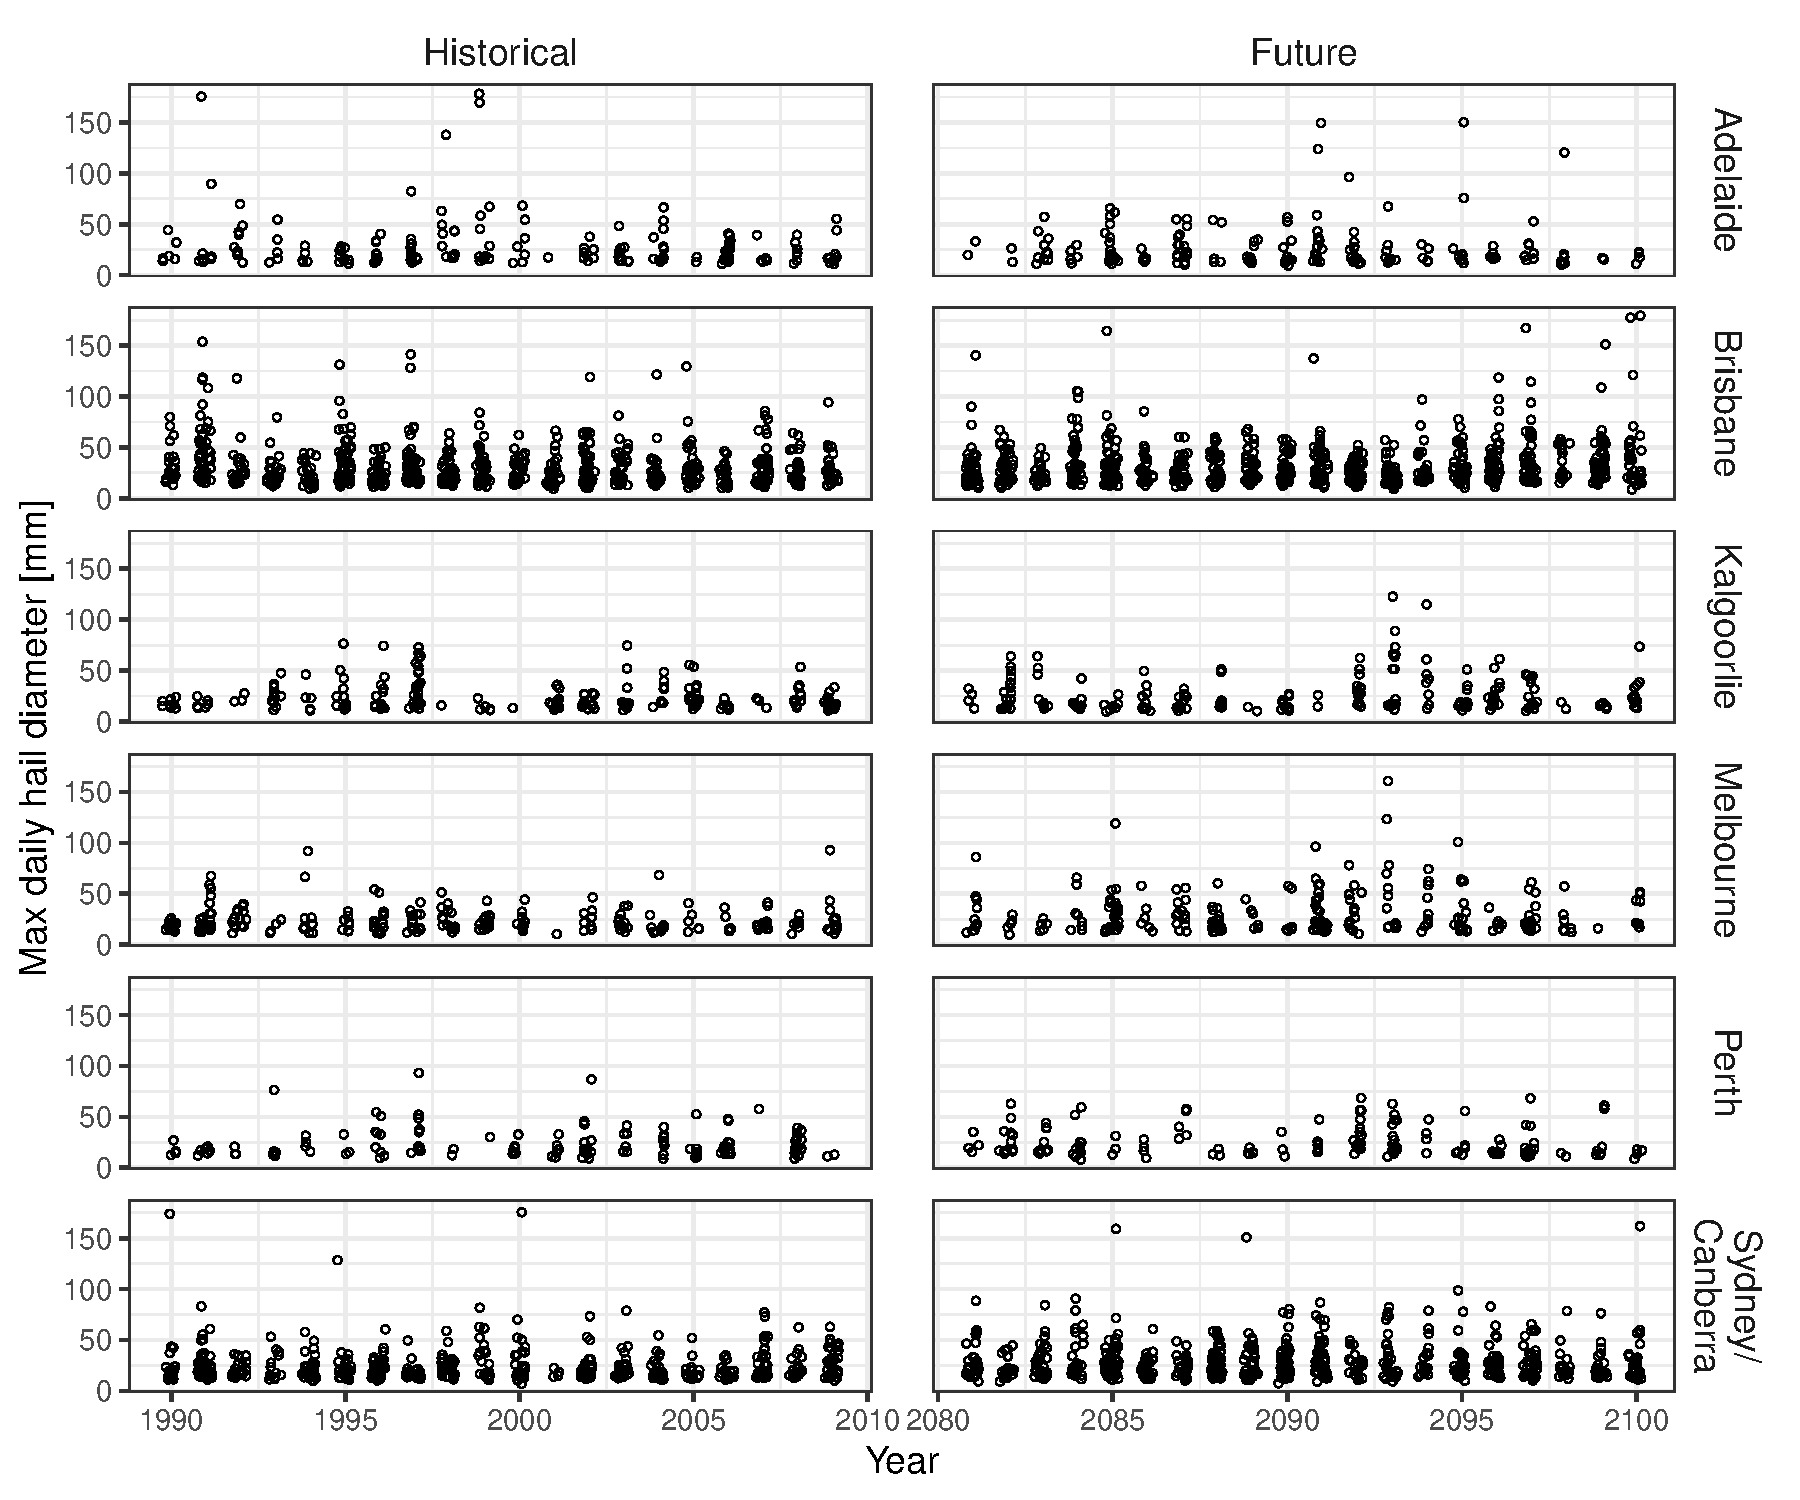
\includegraphics[width=\textwidth]{figures/timeseries_hail}
    \caption{Time series of daily maximum hail sizes by domain and epoch. Gaps exist because only the convective season was simulated each year.}
    \label{fig:timeseries_hail}
\end{figure}

\begin{figure}[!ht]
    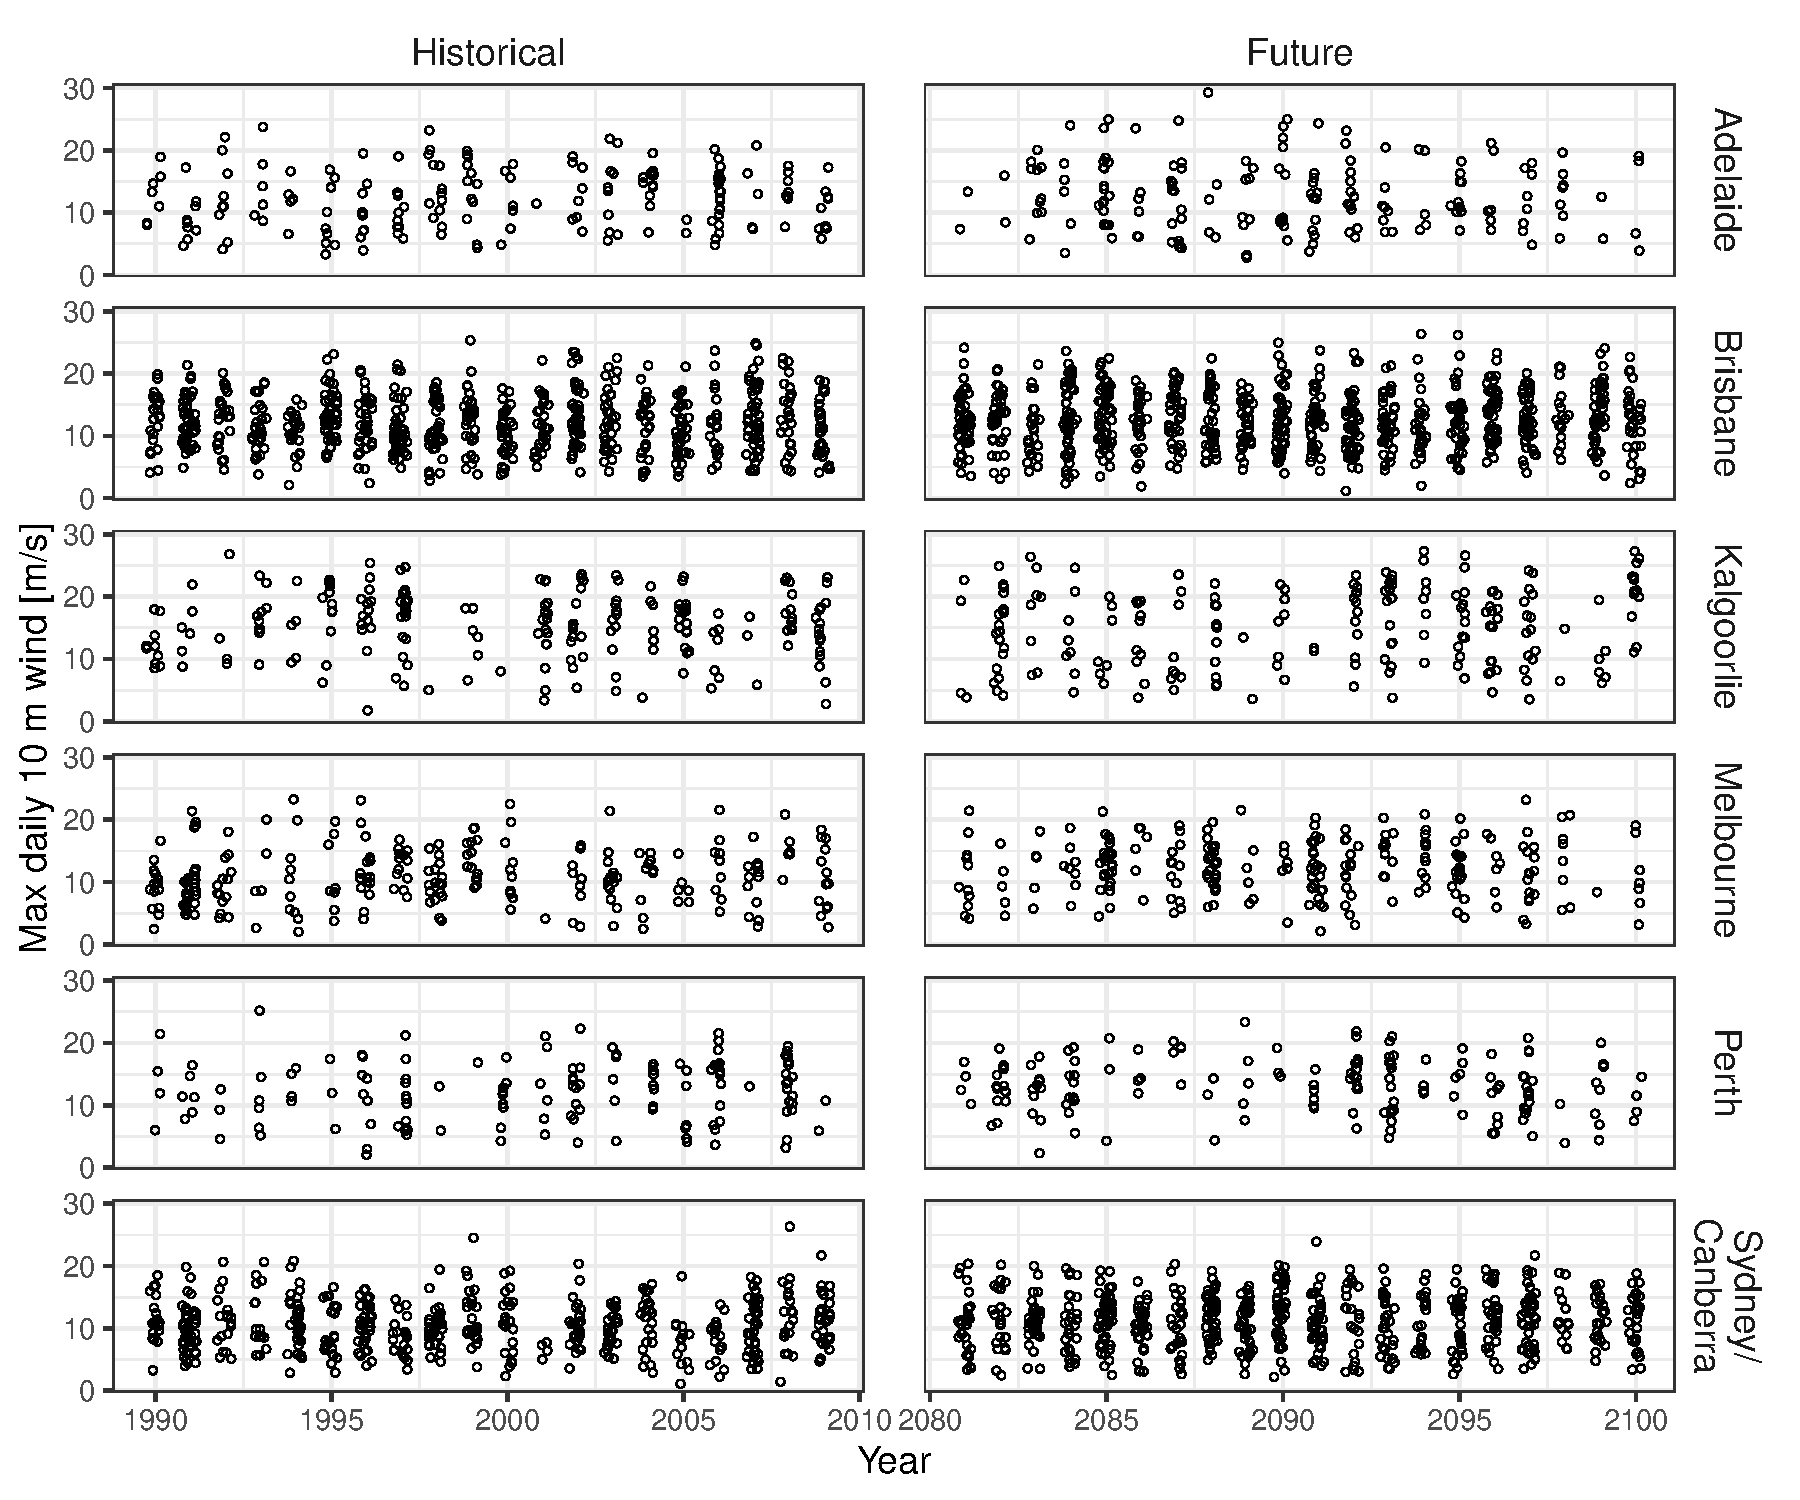
\includegraphics[width=\textwidth]{figures/timeseries_wind}
    \caption{As for Figure \ref{fig:timeseries_hail}, but for daily maximum 10 m wind collocated with hail.}
    \label{fig:timeseries_wind}
\end{figure}

\begin{figure}[!ht]
    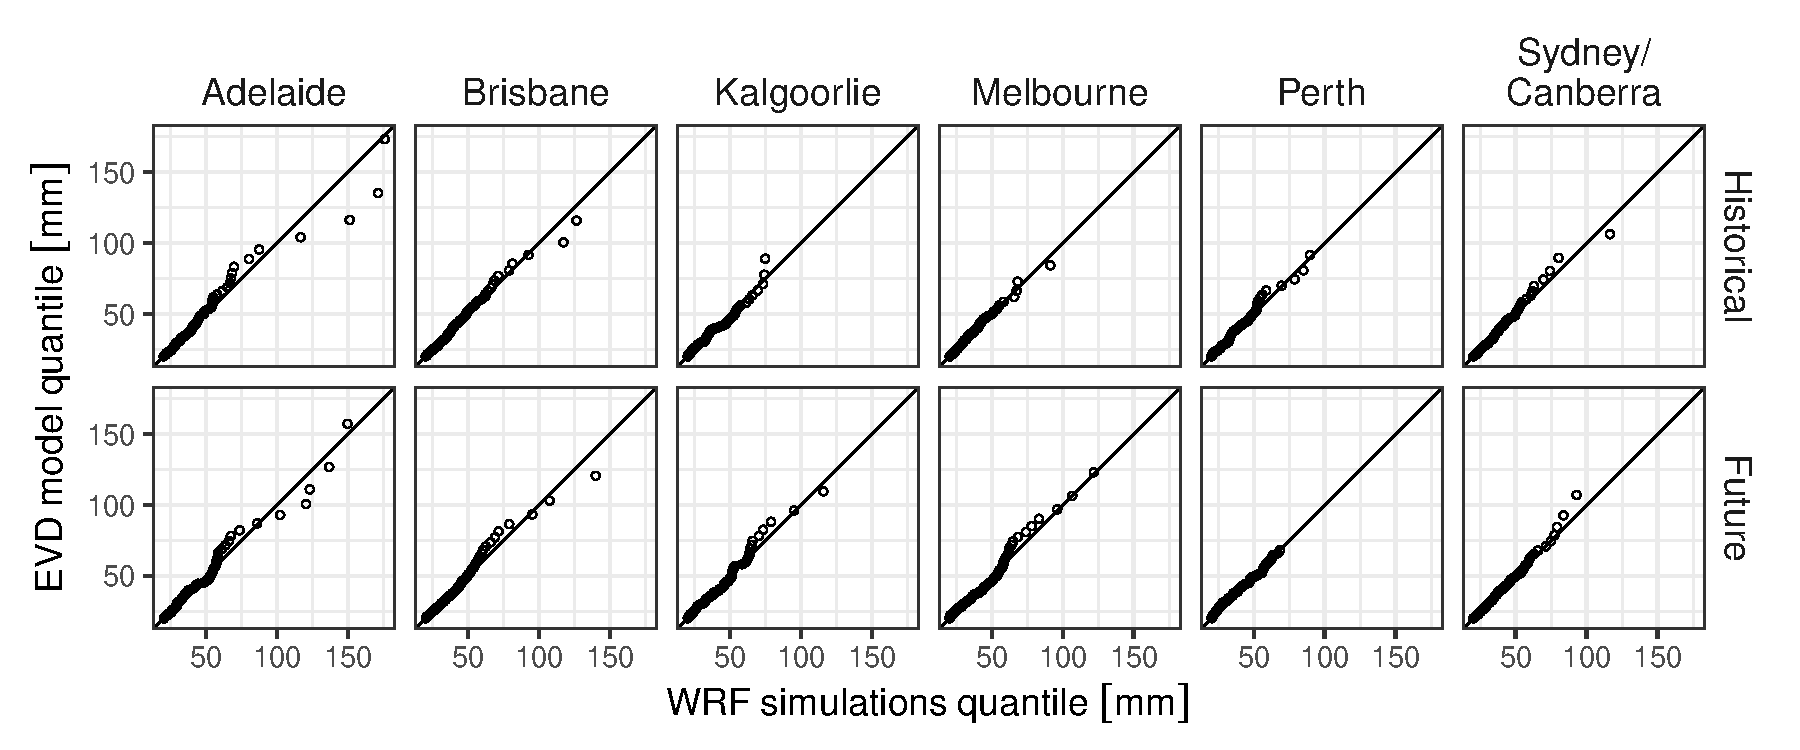
\includegraphics[width=\textwidth]{figures/qq_hail}
    \caption{Quantile-quantile plots for GEV models fitted to daily maximum hail sizes, per domain and epoch.}
    \label{fig:qq_hail}
\end{figure}

\begin{figure}[!ht]
    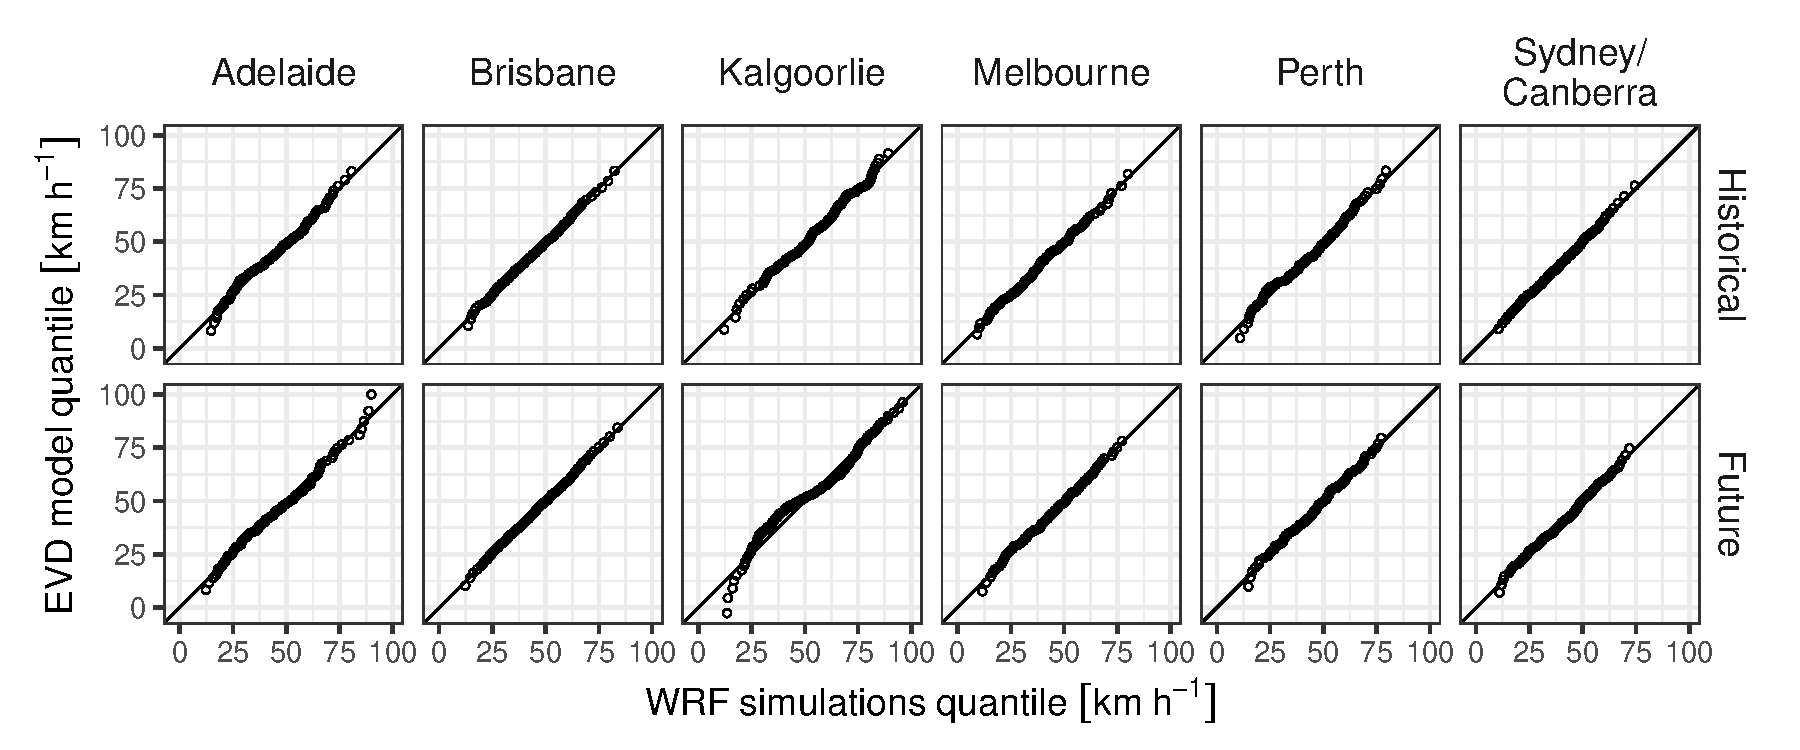
\includegraphics[width=\textwidth]{figures/qq_wind}
    \caption{Quantile-quantile plots for GEV models fitted to daily maximum 10 m wind collocated with hail.}
    \label{fig:qq_wind}
\end{figure}

\begin{figure}[!ht]
    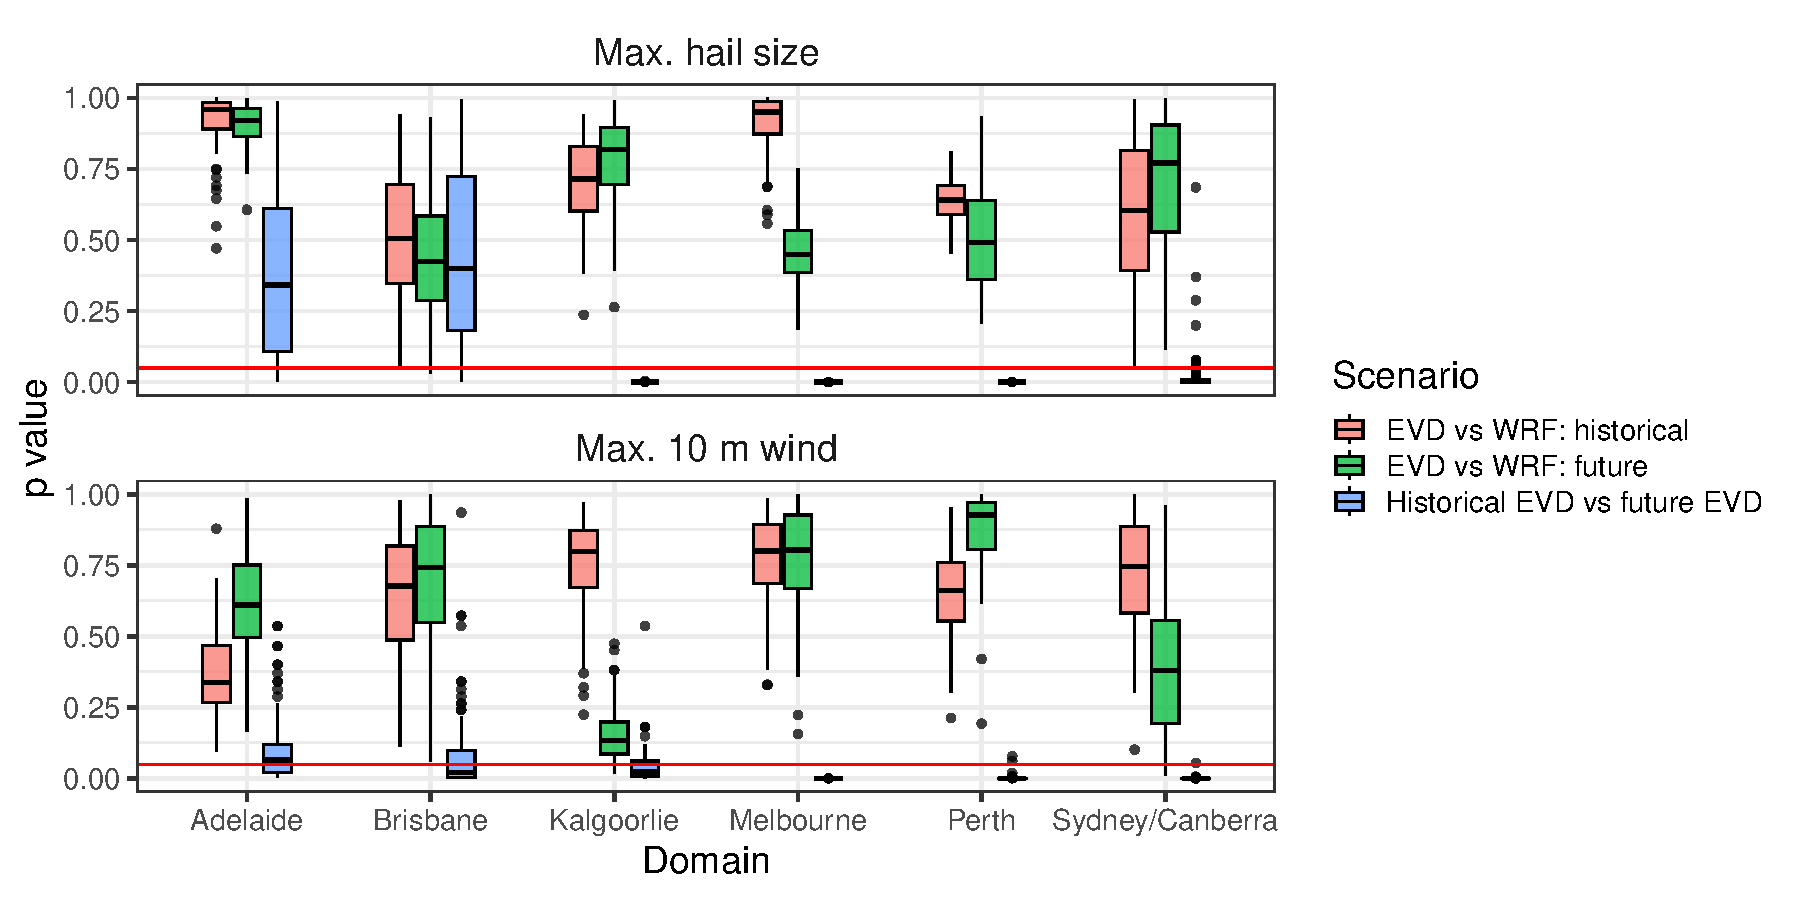
\includegraphics[width=\textwidth]{figures/fit_pvals}
    \caption{Distributions of $p$ values from KS tests, comparing empirical values GEV models, and historical GEVs to future GEVs, per variable and domain. For each test, the KS test was applied 100 times with 1000 random values drawn from the relevant GEV distribution(s) each time, to obtain a distribution of $p$ values. Bars show medians, box hinges show the interquartile ranges (IQRs), whiskers show the largest (smallest) values no more than 1.5 $\times$ IQR from the upper (lower) hinge, and points show outlier points beyond the whisker ranges. The red horizontal line shows $p = 0.05$; when $p$ values are below this line the null hypothesis that the two samples come from the same distribution can be rejected.}
    \label{fig:ks_pvals}
\end{figure}

\clearpage

\begin{table}[!ht]
    \caption{Parameterization schemes used in the WRF simulations.}
    \label{tab:schemes}
    \centering
    \begin{tabular}{lr}
          \hline
          Microphysics & P3-3moment \cite{Milbrandt_JAS_2021} \\
          Cumulus (medium and coarse nests only) & New Tiedtke \cite{Zhang_JC_2017} \\
          Long wave and shortwave radiation & RRTMG \cite{Iacono_JGRA_2008} \\
          Planetary boundary layer & YSU \cite{Hong_MWR_2006} \\
          Surface layer & Revised MM5 \cite{Jimenez_MWR_2012} \\
          Land surface & Noah-MP \cite{Niu_JGRA_2011} \\
          \hline
    \end{tabular}
\end{table}

\begin{table}
    \centering
    \caption{Probability of exceeding hail sizes of 20, 50, or 100 mm, and of coincident wind exceeding 80 and 100 km h$^{-1}$, per domain and epoch.}
    \label{tab:exceedence_probs}
    \begin{tabular}{llccccc}
    \hline
    & & \multicolumn{3}{c}{Hail probability [\%]} & \multicolumn{2}{c}{Wind probability [\%]} \\ 
    Domain & Epoch & 20 mm & 50 mm & 100 mm & 80 km h$^{-1}$ & \multicolumn{1}{c}{100 km h$^{-1}$} \\ 
    \hline
Adelaide & Historical  & $49.99$ & $10.49$ & $\phantom{0}3.45$ & $\phantom{0}1.70$ & $\phantom{0}0.00$ \\ & Future  & $48.70$ & $\phantom{0}9.23$ & $\phantom{0}2.62$ & $\phantom{0}5.41$ & $\phantom{0}1.00$ \\Brisbane & Historical  & $68.34$ & $12.65$ & $\phantom{0}2.48$ & $\phantom{0}1.64$ & $\phantom{0}0.02$ \\ & Future  & $72.17$ & $13.12$ & $\phantom{0}2.30$ & $\phantom{0}2.06$ & $\phantom{0}0.01$ \\Kalgoorlie & Historical  & $43.85$ & $\phantom{0}6.22$ & $\phantom{0}1.51$ & $\phantom{0}9.03$ & $\phantom{0}0.00$ \\ & Future  & $46.79$ & $\phantom{0}8.89$ & $\phantom{0}2.57$ & $13.02$ & $\phantom{0}0.23$ \\Melbourne & Historical  & $45.82$ & $\phantom{0}4.29$ & $\phantom{0}0.65$ & $\phantom{0}1.26$ & $\phantom{0}0.05$ \\ & Future  & $60.50$ & $12.77$ & $\phantom{0}3.66$ & $\phantom{0}0.59$ & $\phantom{0}0.00$ \\Perth & Historical  & $45.57$ & $\phantom{0}6.02$ & $\phantom{0}1.11$ & $\phantom{0}1.84$ & $\phantom{0}0.00$ \\ & Future  & $49.06$ & $\phantom{0}6.98$ & $\phantom{0}1.35$ & $\phantom{0}0.89$ & $\phantom{0}0.00$ \\Sydney/Canberra & Historical  & $49.26$ & $\phantom{0}6.01$ & $\phantom{0}1.04$ & $\phantom{0}0.57$ & $\phantom{0}0.01$ \\ & Future  & $61.83$ & $\phantom{0}9.93$ & $\phantom{0}1.78$ & $\phantom{0}0.24$ & $\phantom{0}0.00$ \\
    \hline 
    \end{tabular}
\end{table}

\end{document}
